\documentclass[a4paper, landscape, 12pt]{article}

\usepackage[left = 2cm, bottom = 3cm, right = 3cm, top = 2cm]{geometry}
\usepackage{pgfplots}

\pagestyle{empty}

\begin{document}
\begin{figure}
    \centering
    \large

    \textit{Laufzeitmessungen und Werte der Formel für $M = 5$ und $1 \le k_i \le 4$}
    \vspace{1.5em}

    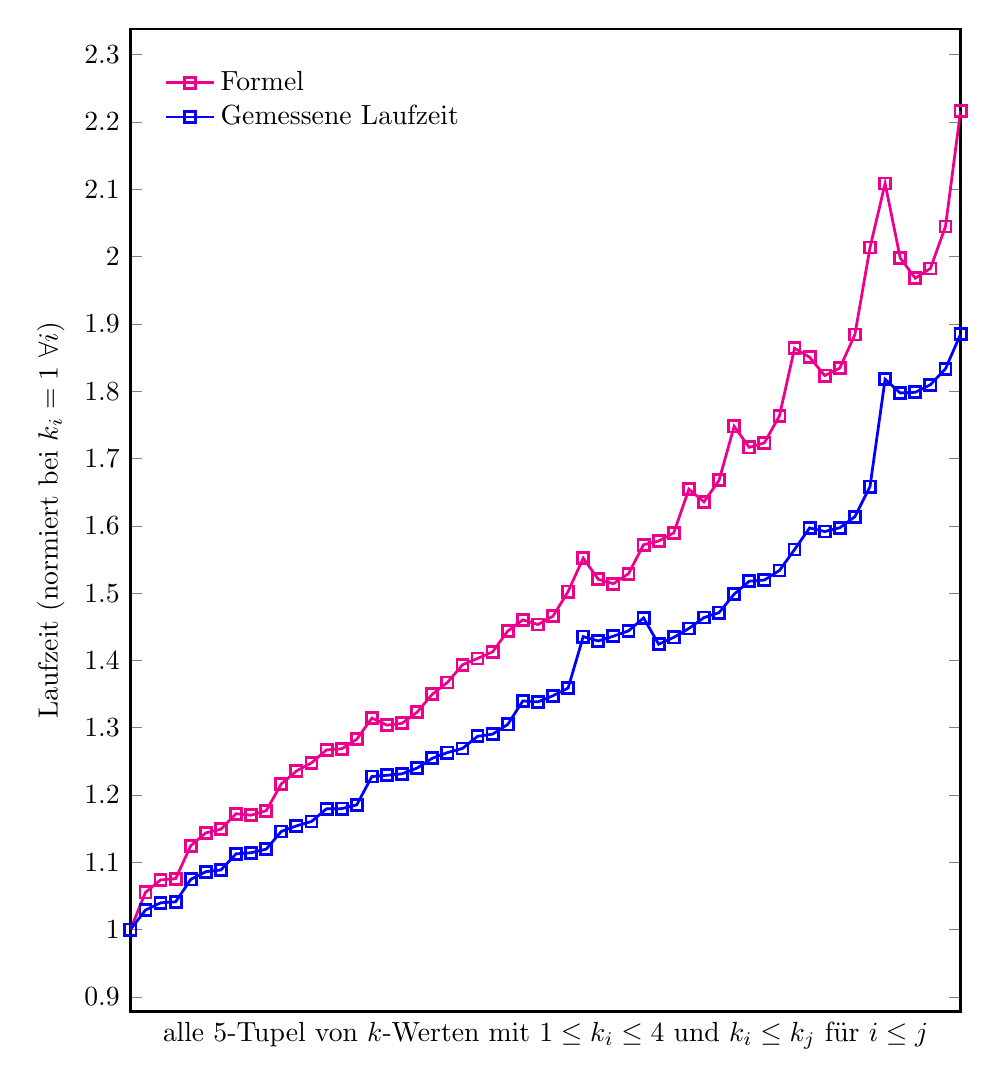
\begin{tikzpicture}
        \begin{axis}[
                xlabel = {alle 5-Tupel von $k$-Werten mit $1 \le k_i \le 4$ und $k_i \le k_j$ für $i \le j$},
                ylabel = {Laufzeit (normiert bei $k_i = 1 \ \forall i$)},
                xmin = 1,
                xmax = 56,
                xmajorticks=false,
                width = \textwidth,
                height = 400pt,
                legend pos = north west,
                legend style = {draw = none},
                legend cell align = left,
                line width = 1pt,
            ]

            \addplot[color = magenta, mark = square]
            coordinates {
                    (1, 1)
                    (2, 1.0553153205892174)
                    (3, 1.0738470260581856)
                    (4, 1.0757019216365709)
                    (5, 1.1246605813619268)
                    (6, 1.1437838591654141)
                    (7, 1.1491919302615723)
                    (8, 1.1721946355004293)
                    (9, 1.1700336727114726)
                    (10, 1.1766895638772126)
                    (11, 1.2165260070098824)
                    (12, 1.2356454328469548)
                    (13, 1.2476997651904118)
                    (14, 1.267048477630227)
                    (15, 1.268653943192539)
                    (16, 1.2829053372046952)
                    (17, 1.3143531516911406)
                    (18, 1.303781353349178)
                    (19, 1.3065376911495508)
                    (20, 1.3232167446601386)
                    (21, 1.3495864094170422)
                    (22, 1.3671964801557446)
                    (23, 1.3933927659371166)
                    (24, 1.4028612422317246)
                    (25, 1.4127448091786787)
                    (26, 1.443670636413471)
                    (27, 1.4602849067656536)
                    (28, 1.4533519114386149)
                    (29, 1.4657842750270573)
                    (30, 1.5022649154565035)
                    (31, 1.5520194838712713)
                    (32, 1.5204990916787047)
                    (33, 1.5139791063363384)
                    (34, 1.5288776314178982)
                    (35, 1.5719285200599413)
                    (36, 1.5773502691896257)
                    (37, 1.5894871706997362)
                    (38, 1.6544582604454825)
                    (39, 1.6356364918167747)
                    (40, 1.6676276287776637)
                    (41, 1.7477805243444966)
                    (42, 1.7165660555059628)
                    (43, 1.7232449640208372)
                    (44, 1.7632884965779283)
                    (45, 1.863818382344943)
                    (46, 1.8505089484747435)
                    (47, 1.823208655868691)
                    (48, 1.8343160783397374)
                    (49, 1.884298459973947)
                    (50, 2.013430336799696)
                    (51, 2.1086517918741277)
                    (52, 1.998094640985621)
                    (53, 1.9679155552562486)
                    (54, 1.9823798942513304)
                    (55, 2.0446787819138668)
                    (56, 2.21648605664914)
                };

            \addplot[color = blue, mark = square]
            coordinates{
                    (1, 1)
                    (2, 1.02905283891897)
                    (3, 1.0397833996393568)
                    (4, 1.0413399495932645)
                    (5, 1.0745966300759886)
                    (6, 1.0860674252857745)
                    (7, 1.0886117231309547)
                    (8, 1.112533337420128)
                    (9, 1.1142318102079236)
                    (10, 1.1195741700125703)
                    (11, 1.1458943394332277)
                    (12, 1.154080101842898)
                    (13, 1.1606769091551818)
                    (14, 1.1797076831359345)
                    (15, 1.1797634518490963)
                    (16, 1.1853997968554213)
                    (17, 1.2274402347822735)
                    (18, 1.2293033275373892)
                    (19, 1.2315435695886694)
                    (20, 1.2400938598600848)
                    (21, 1.254603392437811)
                    (22, 1.2630096992850943)
                    (23, 1.269192371366039)
                    (24, 1.287190404071763)
                    (25, 1.2904869041714897)
                    (26, 1.3049119423356255)
                    (27, 1.3397443002586495)
                    (28, 1.3383858555018777)
                    (29, 1.3475830153528094)
                    (30, 1.3588477132372514)
                    (31, 1.4353672059524125)
                    (32, 1.428908279448792)
                    (33, 1.4359986555759385)
                    (34, 1.4439042185667408)
                    (35, 1.4631522277844171)
                    (36, 1.4241073952671368)
                    (37, 1.4342290783810459)
                    (38, 1.447488317825766)
                    (39, 1.463663103514614)
                    (40, 1.4710319070040865)
                    (41, 1.498438942026172)
                    (42, 1.5177292176011103)
                    (43, 1.5194124236366513)
                    (44, 1.5336127604351475)
                    (45, 1.5647058696760832)
                    (46, 1.5969160026738036)
                    (47, 1.5914801017749778)
                    (48, 1.5971098590206714)
                    (49, 1.6135939119838258)
                    (50, 1.6582772981946199)
                    (51, 1.817747217252669)
                    (52, 1.7974231458503214)
                    (53, 1.7983834575059399)
                    (54, 1.8096433677736437)
                    (55, 1.8333777849716577)
                    (56, 1.8847760704875476)
                };

            \legend{Formel, Gemessene Laufzeit}
        \end{axis}
    \end{tikzpicture}



\end{figure}
\end{document}